\chapter{Fuzzing}

Il fuzzing (o \textit{fuzz testing}) è una tecnica di testing del software 
completamente automatizzata. Il suo approccio si basa sull'invio massiccio e ad 
altissima frequenza (fino a migliaia di test al minuto) di input casuali, malformati 
o inattesi. A differenza del testing tradizionale, il fuzzing non inserisce dati 
"validi" per verificare le normali funzionalità, ma sottopone il sistema a uno 
stress estremo con l'obiettivo di causare crash, blocchi o comportamenti anomali, 
portando così alla luce potenziali vulnerabilità di sicurezza (come i \textit{Buffer Overflow}).

Si tratta di una tecnica estremamente versatile: può essere applicata a qualsiasi 
livello dell'architettura software e hardware che accetti dati in ingresso, partendo 
dai protocolli di comunicazione (come il Bluetooth e i protocolli di rete), passando 
per il sistema operativo, fino ad arrivare a specifiche applicazioni o browser web.

Dal punto di vista operativo, il fuzzing si comporta a tutti gli effetti come un 
approccio a forza bruta. Generando una quantità enorme di dati, richiede una 
notevole potenza di calcolo, tanto che spesso vengono impiegati interi datacenter 
dedicati. Proprio per la sua efficacia, le grandi aziende tech come Google e Microsoft 
investono pesantemente in questa attività per testare i propri applicativi: data 
l'ampia diffusione dei loro prodotti, individuare e risolvere preventivamente 
vulnerabilità critiche è di fondamentale importanza.

\section{Test Positivo vs Test Negativo}

Nella tradizionale ingegneria del software, il testing funzionale (o positivo) 
verifica che il software faccia ciò per cui è stato progettato, controllando la 
conformità ai requisiti e le performance. Si tratta dunque di un'attività principalmente
manuale. 

Il fuzzing implementa invece il test negativo: esplora lo spazio degli input "non 
definiti" per garantire che il software non manifesti comportamenti pericolosi 
(crash, stalli, command injection, information leaks) quando riceve dati imprevisti.
I bug di sicurezza spesso risiedono in "\textit{feature creative}" o nella gestione 
errata della memoria quando il software tenta di processare formati malformati. 
Inviando lunghezze non valide, messaggi fuori sequenza (\textit{out-of-state}), o causando 
overflow/underflow, si forza l'applicazione fuori dal suo normale flusso di controllo.

Nel panorama del fuzzing, l'automazione gioca un ruolo centrale su due fronti 
fondamentali del testing: la generazione degli input e la validazione dei risultati.

Da un lato, il tool di fuzzing si occupa autonomamente di generare massicce quantità 
di dati casuali o malformati. Dall'altro, il ruolo del cosiddetto "\textbf{oracolo}", 
ovvero il componente deputato a stabilire se il test sia fallito o meno, è ricoperto 
dai \textbf{sanitizer}. A differenza dei test funzionali classici, che verificano il 
rispetto di requisiti positivi, i sanitizer si fondano per loro natura su requisiti 
negativi: il loro scopo è intercettare e segnalare tutto ciò che il sistema non deve 
assolutamente fare, come violare i limiti di memoria o bloccarsi in modo anomalo.

Questa architettura permette di sfruttare framework di fuzzing già esistenti e pronti 
all'uso. Avviando uno di questi tool, sarà il sistema stesso, supportato dai sanitizer 
integrati, a notificarci automaticamente l'eventuale innesco di vulnerabilità 
specifiche, come un Buffer Overflow, a seguito dei test eseguiti.

Il grande vantaggio concettuale e operativo del fuzzing risiede proprio in questo: 
semplifica drasticamente l'attività di testing poiché delega completamente al tool sia 
la complessa generazione dei dati di ingresso (\textbf{input}), sia la definizione e il 
controllo delle condizioni di anomalia (\textbf{output atteso}).

\section{Tipi di Fuzzer}

\begin{itemize}
    \item \textbf{Puramente random}: funziona bene solamente se il software è 
    particolarmente vulnerabile, altrimenti risulta poco efficace specialmente nel 
    caso di software robusti.
    \item \textbf{Generation-based}: non è casuale, è basato su un modello dell'applicativo 
     da testare. I messaggi da creare sono più realistici poichè generati da un 
     algoritmo specifico.
    \item \textbf{Mutation-based}: partendo da un input valido si va a "sporcare" un 
    pezzetto di quell'input valido creando così un "mutante".
\end{itemize}

A prescindere dalla specifica architettura del Fuzzer impiegato, il ciclo di vita 
dell'input generato attraversa una serie di filtri sequenziali. Affinché un test sia 
realmente efficace e vada a stimolare le vulnerabilità interne del software, l'input 
deve superare i controlli superficiali e raggiungere la logica profonda dell'applicativo, 
il che avviene tipicamente al terzo step di validazione.

Il primo ostacolo è il controllo della \textbf{sintassi}. Se il Fuzzer genera dati 
completamente malformati o "spazzatura", questi falliranno per sintassi invalida. Il 
parser del sistema rileverà immediatamente l'errore di formattazione e scarterà l'input, 
impedendogli di procedere oltre.

Il secondo livello riguarda il controllo della \textbf{semantica}. In questo caso, 
l'input generato ha superato i controlli sintattici, ma risulta logicamente o 
contestualmente errato. Si parla di semantica invalida quando, ad esempio, l'input è 
ben formattato ma omette un parametro richiesto obbligatoriamente dalle regole di 
business del software (come fornire il campo \textit{USER} ma tralasciare il campo 
\textit{PASS} in una procedura di autenticazione). Anche in questo scenario, il test 
si arresta prematuramente.

L'ultimo step si raggiunge solo quando l'input presenta \textbf{sia sintassi che semantica 
valide}. In questa fase cruciale, il dato malevolo o inatteso viene finalmente dato in 
pasto al "core" del software. Generare input in grado di raggiungere questo livello è 
il vero e proprio obiettivo di un'attività di Fuzzing avanzata: è solo superando le 
barriere di validazione iniziale che si ottiene un test ad alto valore aggiunto, 
capace di mandare in crash l'applicativo e scovare vulnerabilità profonde e critiche.

\subsection{Generation-based Fuzzers (Fuzzing Generazionale)}

Questi fuzzer si basano su un modello formale del protocollo da testare (es. Automi a Stati Finiti - FSM). 
Navigano nel modello generando prima pacchetti validi per superare i controlli 
iniziali (es. l'autenticazione), per poi iniettare corruzioni negli strati più profondi.

\begin{figure}[H]
    \centering
    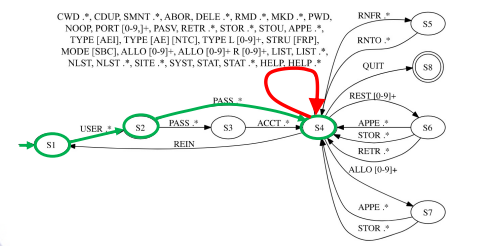
\includegraphics[width=0.7\linewidth]{img/capitolo6/generation.png}
    \label{fig:generation}
\end{figure}

\begin{itemize}
    \item \textbf{Vantaggi}: Raggiungono stati di protocollo più profondi in meno tempo.
    \item \textbf{Svantaggi}: Richiedono un esperto per modellare le specifiche (RFC) e scrivere il fuzzer.
    Inoltre spesso i prodotti che vogliamo testare non rispettano mai al 100\% 
    gli standard dei vari protocolli, quindi non è detto che pur avendo un modello 
    fatto bene questo sia efficace su tutti i prodotti da testare.
\end{itemize}

Esempio pratico (\textbf{Metasploit}): Metasploit non è un fuzzer, è un tool avente un 
grosso DB di exploit; tuttavia al suo interno ha anche dei piccoli fuzzer. Si tratta di
fuzzer generation-based quindi studiati in base al protocollo da testare; se il 
protocollo che ci interessa non è presente significa che Metasploit non lo copre.
Nel seguente esempio è stato usato il fuzzer per il protocollo FTP (\textit{ftp\_pre\_post})
ed è stato lanciato contro un server target. Il fuzzer viene configurato con uno step 
incrementale di 100 byte (\textit{STEPSIZE 100}) e si osserva l'invio di pattern ciclici
sempre più grandi: 10, 110, 210... fino a 2110 byte.

\begin{figure}[H]
    \centering
    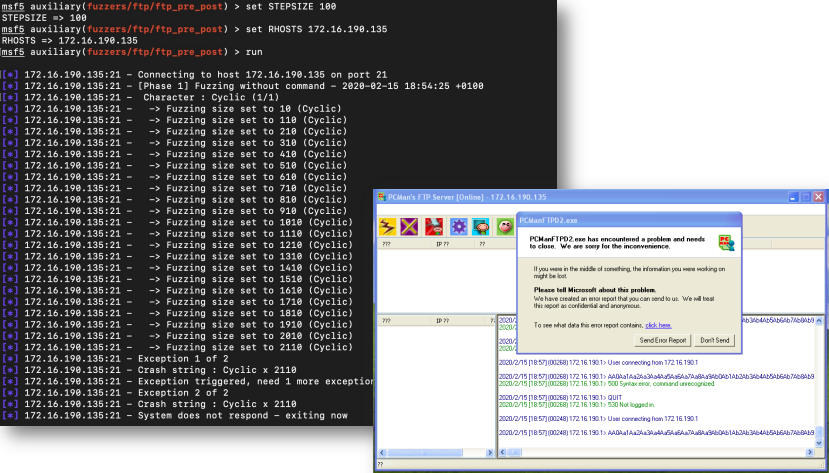
\includegraphics[width=1\linewidth]{img/capitolo6/metasploit.png}
    \label{fig:metasploit}
\end{figure}

A 2110 byte, l'output segnala "Exception 1 of 2" e il processo "PCManFTPD2.exe" sul 
target va in errore e si chiude.
La stringa generata da Metasploit è un pattern de Bruijn (visibile nel debugger log: 
Aa8Aa9Ab0Ab1...). Quando il server tenta di copiare questa enorme stringa in un buffer 
locale allocato nello stack (magari destinato a soli 512 byte), i dati in eccesso 
sovrascrivono i metadati di controllo dello stack. Il crash avviene perché la CPU 
tenta di eseguire codice all'indirizzo sovrascritto.

Esempio pratico (\textbf{Sulley}): Si tratta di un tool di fuzzing scritto in Python. 
Scopo nostro in questo caso è testare ancora il protocollo FTP; si configura l'IP, il 
numero di porto e altre impostazioni di configurazione. Ma come creiamo la macchina a 
stati finiti che descriva il modello del protocollo di interesse? Prima di tutto inizializziamo i 
campi "user" e "pass":

\begin{lstlisting}
s_initialize("user")
s_string("USER", fuzzable=False)
s_delim(" ", fuzzable=False)
s_string("anonymous", fuzzable=False)
s_static("\r\n")
s_initialize("pass")
s_string("PASS", fuzzable=False)
s_delim(" ", fuzzable=False)
s_string("james", fuzzable=False)
s_static("\r\n")
\end{lstlisting}

Da notare che i parametri \textit{fuzzable} qui sono \textbf{False}: questo garantisce 
che l'autenticazione vada sempre a buon fine. Il fuzzing vero e proprio avverrà su 
comandi successivi, come \textbf{LS} o \textbf{RECV}, dove i fuzzer inietteranno 
stringhe anomale per corrompere la memoria o tentare un Path Traversal.

\begin{lstlisting}
s_initialize("list")
s_string("LS")
s_delim(" ")
s_string("AAAA")
s_static("\r\n")
s_initialize("recv")
s_string("RECV")
s_delim(" ")
s_string("AAAA")
s_delim(" ")
s_string("BBBB")
s_static("\r\n")
\end{lstlisting}

Ultimo step è creare la macchina a stati finiti andando a collegare i vari messaggi 
tra di loro:

\begin{lstlisting}
session.connect(s_get("user"))
session.connect(s_get("user"), s_get("pass"))
session.connect(s_get("pass"), s_get("list"))
session.connect(s_get("pass"), s_get("recv"))
session.fuzz()
\end{lstlisting}

\subsection{Mutation-based Fuzzers (Fuzzing Mutazionale)}

Questi fuzzer partono da un input iniziale valido, chiamato \textbf{seed} (ad esempio 
un file pcap di traffico di rete o un'immagine), e lo mutano inserendo anomalie.

\begin{itemize}
    \item \textbf{Vantaggi}: Richiedono pochissimo sforzo e non necessitano di competenze specifiche sul protocollo.
    \item \textbf{Svantaggi}: La copertura del codice è limitata dal seed iniziale; 
    sono incapaci di raggiungere bug "profondi" perché le mutazioni casuali spesso 
    distruggono la sintassi di base, facendo sì che il target scarti il pacchetto 
    subito.
\end{itemize}

Esempio pratico (\textbf{Mutiny Fuzzer}): Mutiny prende un traffico di rete legittimo 
(es. una sessione FTP registrata in un file PCAP con comandi validi come USER 
\textit{anonymous} e PASS \textit{aaaa}) e lo usa come seed. Utilizza uno script 
(\textit{mutiny\_prep.py}) per generare un file .fuzzer di configurazione e poi avvia 
l'attacco riproducendo il traffico alterato verso l'IP bersaglio.

\section{Fuzzing basato su Algoritmi Genetici}

I fuzzer tradizionali spesso falliscono con protocolli di rete o formati di file 
complessi perché generano input casuali che vengono immediatamente scartati dai 
controlli di validità iniziali del programma. Gli algoritmi genetici risolvono 
questo problema applicando mutazioni evolutive a input validi noti. Il fuzzer 
modella i dati seguendo una gerarchia:

\begin{itemize}
    \item \textbf{Token}: Una singola unità di dato (es. una stringa o un numero).
    \item \textbf{Session} (o \textbf{Leg}): Un'intera transazione o sequenza di comandi 
    inviati al target.
    \item \textbf{Pool}: Un gruppo di sessioni.
\end{itemize}

\begin{figure}[H]
    \centering
    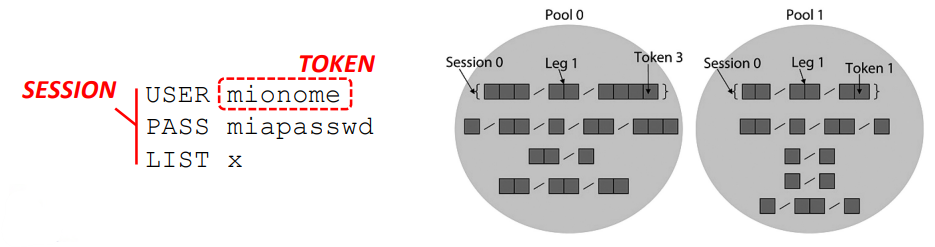
\includegraphics[width=1\linewidth]{img/capitolo6/input.png}
    \label{fig:input}
\end{figure}

A ogni "generazione", gli input vengono mescolati e alterati per massimizzare una 
funzione di \textit{fitness} (es. la quantità di stati del protocollo o codice 
esplorato).

\begin{itemize}
    \item \textbf{Crossover}: Due sessioni ad alta fitness vengono combinate 
    tagliandole in un punto casuale e scambiando i segmenti. Ad esempio, date due 
    sessioni $A=A_1 + A_2$ e $B=B_1 + B_2$, il crossover genera i figli $A'=A_1 + B_2$
    e $B'=A_2 + B_1$.
    \item \textbf{Mutazione}: Singoli token all'interno di una sessione vengono 
    alterati casualmente (es. inserendo stringhe di formato vulnerabili come \%n\%n). 
    Lo stesso principio si applica ai pool, aggiungendo o rimuovendo intere sessioni.
\end{itemize}

L'idea alla base è che, valutando e selezionando continuamente gli input "migliori" 
generati durante il processo, la fitness globale dei test continui ad aumentare. 
Tuttavia, questo processo non è in grado di fare miracoli da solo: l'efficienza 
dell'intero ciclo dipende in modo critico dalla qualità dei seed iniziali, ovvero i 
dati di partenza forniti al fuzzer. 

Durante questa esecuzione massiva, ogni volta 
che un input causa il crash dell'applicativo, il fuzzer salva automaticamente 
quell'istanza. Questa archiviazione è fondamentale perché permette di replicare e 
analizzare il crash in un secondo momento, identificando l'esatta vulnerabilità che 
lo ha scatenato (come, ad esempio, un \textit{Buffer Overflow}). 

Ma come fa il tool a misurare la "qualità" di un test in modo completamente automatico per decidere se 
un input è migliore di un altro? La metrica standard utilizzata è la \textbf{Code Coverage}. 
L'obiettivo primario del fuzzer è proprio quello di massimizzare questa metrica, 
esplorando percorsi di esecuzione sempre nuovi. Per sua natura logica, l'andamento 
della coverage nel tempo è descrivibile come una funzione monotona non decrescente: 
all'aumentare dei test eseguiti, la porzione di codice esplorata può solamente 
aumentare o, nel peggiore dei casi, restare invariata, ma non potrà mai diminuire. 

A livello tecnico, la misurazione della coverage non avviene quasi mai contando le 
singole righe di codice, bensì ragionando per \textbf{Code Block}. Un Code Block è una 
sequenza lineare di istruzioni indivisibili dal punto di vista del flusso di 
controllo: se il programma inizia a eseguire la prima istruzione del blocco, 
eseguirà necessariamente anche tutte le successive fino alla fine del blocco stesso.

Per tracciare il passaggio attraverso questi blocchi, il codice viene sottoposto a 
\textbf{strumentazione} (spesso tramite i sanitizer o il compilatore stesso). Un 
metodo implementativo classico consiste nel creare un array di $n$ posizioni (dove $n$ 
rappresenta il numero totale di Code Block del programma) inizializzato a \textit{False}. 
All'interno di ogni blocco viene iniettata una piccola istruzione di tracciamento: 
non appena il flusso di esecuzione attraversa quel blocco, la posizione 
corrispondente nell'array viene impostata su \textit{True}, segnalando al fuzzer che 
quella specifica porzione di codice è stata coperta con successo.

\textbf{Classificazione dei Fuzzer}

\begin{itemize}
    \item \textbf{Black-box}: Nessuna conoscenza interna; si basano solo su input e output/crash.
    \item \textbf{Grey-box}: Raccolgono informazioni limitate sulla struttura del programma (come la copertura di istruzioni e rami) tramite analisi statica leggera e strumentazione.
    \item \textbf{White-box}: Analizzano profondamente la struttura interna (esecuzione simbolica, taint analysis), ma sono computazionalmente pesanti.
\end{itemize}

\subsection{American Fuzzy Lop (AFL)}

AFL è il fuzzer grey-box guidato dalla copertura per eccellenza. Richiede un 
programma target eseguibile e funziona modificando file in input per esplorare nuovi 
percorsi di esecuzione.

Per comprendere la potenza di tale fuzzer riportiamo un esempio che riguarda un parser JPEG:
il file di input iniziale è un semplice file di testo contenente la parola "hello", tuttavia,
AFL essendo guidato dalla copertura capisce che modificando il primo byte in \textit{0xFF}, il 
parser JPEG esegue un ramo di codice diverso. Successivamente, AFL indovina \textit{0xFF 0xD8}
(cioè l'header valido di un JPEG) e, nel giro di 1-2 giorni di esecuzione su 4 core,
riesce a generare un'immagine JPEG strutturalmente valida esclusivamente mutando la 
parola "hello" e osservando il feedback del programma.

\textbf{Flusso di lavoro con AFL}

\textbf{1. Preparazione e Strumentazione del codice}: Il primo passo consiste nel 
ricompilare il codice sorgente del programma bersaglio. Non si utilizza un 
compilatore standard, bensì un wrapper fornito dal tool stesso, come \textit{afl-gcc}. 
Questo passaggio è cruciale perché inietta nel codice binario la "strumentazione" 
necessaria per misurare la code coverage durante l'esecuzione. Inoltre, per 
facilitare l'individuazione di vulnerabilità legate alla memoria, è prassi comune 
abilitare \textbf{AddressSanitizer} passando la variabile d'ambiente \textit{AFL\_USE\_ASAN=1} 
durante la compilazione.

\textbf{2. Configurazione e Avvio}: Una volta ottenuto l'eseguibile strumentato, si 
raccolgono degli input validi di partenza (i seed) e li si inserisce in una cartella 
dedicata. L'esecuzione del fuzzer si avvia con un comando dalla struttura simile a 
questa:
\begin{gather*}
    \text{afl-fuzz -m none -i <input\_dir> -o <output\_dir> -- ./eseguibile @@}
\end{gather*}

Analizzando i parametri:

\begin{itemize}
    \item \textbf{-m none}: disabilita i limiti di memoria imposti da AFL al programma testato.
    \item \textbf{-i} e \textbf{-o}: indicano rispettivamente le cartelle contenenti i seed di input e dove verranno salvati gli output/crash.
    \item \textbf{@@}: è un segnaposto che indica ad AFL dove inserire il percorso del file temporaneo generato ad ogni iterazione, che verrà passato come input al programma.
\end{itemize}

\textbf{3. Il Motore di Mutazione}: AFL prende i seed iniziali, li inserisce in una 
coda e, ciclicamente, applica diverse strategie di mutazione per generare nuovi input. 
Tra le tecniche principali troviamo:

\begin{itemize}
    \item \textbf{Bit/Byte flip}: inversione mirata di singoli bit o byte.
    \item \textbf{Simple arithmetics}: banali addizioni o sottrazioni sui valori esadecimali.
    \item \textbf{Known integers}: inserimento di valori limite noti per causare errori (es. 0, -1, interi massimi).
    \item \textbf{Splicing}: operazione di crossover che combina frammenti di due input diversi.
    \item \textbf{Stacked}: applicazione combinata e in cascata di più mutazioni.
\end{itemize}

\textbf{4. Misurazione della Fitness}: Ad ogni esecuzione, AFL valuta la qualità 
dell'input generato (la sua fitness) basandosi sulla \textbf{Branch Coverage} 
(copertura dei rami). A differenza della semplice copertura delle singole linee di 
codice, la branch coverage traccia gli archi attraversati nel Control Flow Graph del 
programma. Questa scelta non è casuale: l'esperienza dimostra che le vulnerabilità 
si annidano spesso in stati di transizione imprevisti o mal gestiti.

Per tenere traccia del percorso, AFL utilizza una \textbf{Hit Counter Bitmap} (un 
vettore di bit). Quando il flusso di esecuzione attraversa un determinato "ramo", la 
posizione corrispondente nella bitmap viene segnata come "toccata". Se un input 
appena mutato tocca una parte del grafo che non era mai stata esplorata prima, 
l'input viene considerato "interessante" e viene reinserito nella coda per subire 
ulteriori mutazioni, guidando così l'evoluzione del testing verso percorsi sempre 
più profondi.

\textbf{5. Gestione dei Crash e Deduplicazione}: Se un input causa un crash 
dell'applicativo, questo non viene scartato, ma viene salvato nella sottocartella 
\textit{crashes} all'interno della directory di output. Per ogni crash salvato, AFL 
registra un identificativo, un timestamp e la specifica catena di mutazioni che lo 
ha generato.

È fondamentale sottolineare che \textbf{il numero di crash rilevati non equivale al numero 
di vulnerabilità effettive}. Per limitare il rumore, AFL esegue una deduplicazione 
automatica: confronta la bitmap del nuovo crash con quelle dei crash precedenti. Se 
il nuovo input anomalo ha percorso esattamente gli stessi branch (stessa bitmap) di 
un crash già noto, AFL deduce che la vulnerabilità sottostante sia la medesima e lo 
considera ridondante, evitando di salvarlo come un nuovo unicum.

Infine, per capire l'esatta natura della vulnerabilità scovata, i file salvati nella 
cartella \textit{crashes} vengono presi e dati in pasto all'eseguibile (idealmente 
compilato con ASAN) al di fuori del fuzzer, oppure analizzati passo-passo tramite un 
debugger come \textbf{GDB}.